\section{Анализ литературных источников, прототипов и формирование требований к проектируемому программному средству}
\label{sec:analysis}

Конечный успех программного проекта во многом определяется до начала конструирования: на этапе подготовки, которая проводится с учетом всех особенностей проекта.

Первое предварительное условие, которое нужно выполнить перед конструированием, -- ясное формулирование проблемы, которую система должна решать. Общая цель подготовки — снижение риска: адекватное планирование позволяет исключить главные аспекты риска на самых ранних стадиях работы, чтобы основную часть проекта можно было выполнить максимально эффективно. 

Главный факторы риска в создании ПО — неудачная выработка требований. Требования подробно описывают, что должна делать программная система. Внимание к требованиям помогает свести к минимуму изменения системы после начала разработки \cite{code_complete}.

Перед формулированием требований необходимо изучить ряд вопросов, которые напрямую влияют на все дальнейшие этапы разработки. В частности, необходимо рассмотреть вопросы выбора платформ, архитектуры. По результатам анализа можно будет составить техническое задание к проектируемому программному средству, которое станет основой для составления функциональных требований.

\subsection{Аналитический обзор литературных источников}
\label{sec:analysis:literature}

Далее приводится анализ сведений, которые влияют на формулирование требований, выбор архитектуры и дальнейшее 
проектирование и разработку программного средства.

\subsubsection{} Кроссплатформенность приложений
\label{sec:analysis:literature:crossplatform}

Как несколько десятилетий назад, так и в настоящее время выбор платформы является серьезным ограничением для всех
последующих этапов разработки. Однако уже начали появляться технологии, которые позволяют использовать однажды
написанный код на многих платформах. Сегодня все больше приложений создается сразу для нескольких платформ, а
приложения, созданные изначально для одной платформы, активно адаптируются под другие \cite{habr_crossplatform}.
Разработчик, изучающий какую-либо из таких технологий, получает конкурентное преимущество, поскольку за счет расширения
количества платформ расширяется круг задач, над которыми он может работать. Поэтому кроссплатформенность – реальная или
потенциальная – является одним из факторов, который необходимо учитывать при выборе технологий реализации проекта.

\subsubsection{} Обзор целевых платформ
\label{sec:analysis:literature:platforms}

Несмотря на планируемое использование кроссплатформенных технологий, поддержка всех платформ может затребовать
значительно больших средств и времени, чем есть в наличии для выполнения дипломного проектирования. Поэтому, необходимо
осуществить выбор одной основной платформы с расчетом на продолжение разработки и реализацию проекта для других платформ.
Рассмотрим достоинства и недостатки основных.

Настольное приложение -- программное средство, которое запускается локально на компьютере пользователя. При его
создании появляется возможность использования всех преимуществ аппаратного обеспечения, которым оснащен компьютер,
например: прямой доступ к видеокарте, внешним устройствам. Кроме того, появляется возможность взаимодействия с другими
установленными приложениями.

Тем не менее у настольных приложений есть и ряд недостатков. Когда пользователь работает удаленно, возникают проблемы,
связанные с сетью, соединениями, сетевыми экранами. Один из самых больших недостатков заключается в огромной
сложности развертывания приложения на десятки или сотни машин, их конфигурирования, периодического обновления \cite{msdn_desktop_vs_web}.

Веб-приложения, в отличие от настольных, работают на удаленном аппаратном обеспечении и поставляются пользователю
через браузер \cite{web_based_vs_desktop}. При их использовании разработчик избавляется от необходимости поддерживать
установку большого числа зависимостей, он всегда может быть уверен, что все пользователи используют самую последнюю
версию приложения. Вычислительные операции могут производиться на мощном сервере, а результаты вычислений поставляться
пользователю – так называемая концепция «тонкого клиента» \cite{desktop_vs_web_deeper_look}.

Несмотря на то, что ресурсоемкие вычисления производятся на сервере, задержки при передаче, особенно при нестабильном
соединении, сама потребность в постоянном интернет соединении могут значительно снизить удобство пользования
приложением. Кроме того, размер загружаемого при каждом запуске кода и ресурсов может значительно увеличить траты
пользователя, особенно если он использует дорогое мобильное подключение к интернету.

Для мобильных приложений актуальны ограничения платформ, на которых они запускаются, такие как меньшие размеры
экранов, более медленные процессоры, ограниченное энергопотребление. Несмотря на это, мобиль ные устройства часто
находятся рядом с пользователями, появляется возможность использования мгновенных оповещений \cite{desktop_mobile_differences}.
Вместе с этим, большинство смартфонов оснащено модулями, такими как GPS, камера, NFC, что предоставляет разработчику
новые возможности по их использованию.

На основании рассмотренных характеристик различных платформ можно осуществить выбор одной из них, которая и станет
целевой для разработки.

\subsubsection{} Обзор архитектурных стилей
\label{sec:analysis:literature:architecture}

Далее необходимо рассмотреть применяющиеся на практике архитектурные стили, провести их анализ и по результатам
осуществить выбор архитектуры, которая затем будет применяться при проектировании программного средства.

Под разработкой архитектуры понимают специфицирование структуры всей системы: глобальную организацию и структуру
управления, протоколы коммуникации, синхронизации и доступа к данным, распределение функциональности между компонентами
системы, физическое размещение, состав системы, масштабируемость и производительность \cite{introduction_to_architecture}.
Набор принципов, используемых в архитектуре, формирует архитектурный стиль. Применение архитектурных стилей
упрощают решение целого класса абстрактных проблем \cite{architecture_volosevich}.

При проектировании архитектуры программной системы почти никогда не ограничиваются единственным архитектурным стилем,
поскольку они могут предлагать решение каких-либо проблем в различных областях.
В таблице~\ref{table:analysis:architectures:categorization} приведен вариант категоризации архитектурных
стилей \cite{application_architecture_guide}.

\begin{table}[ht]
  \caption{Категоризация архитектурных стилей}
  \label{table:analysis:architectures:categorization}
  \centering
  \begin{tabular}{|>{\raggedright}m{0.27\textwidth} 
                  |>{\raggedright\arraybackslash}m{0.675\textwidth}|}
    \hline Категория & Архитектурный стиль\\
    \hline Связь & SOA (Service-oriented architecture -- архитектура, ориентированная на сервисы), Шина сообщений\\
    \hline Развертывание & Клиент-серверный, трехуровневый, N-уровневый\\
    \hline Предметная область & DDD (Domain-driven design -- проблемно-ориентированное проектирование)\\
    \hline Структура & Компонентный, объектно-ориентированный, многоуровневый\\
    \hline
  \end{tabular}
\end{table}

Сервис-ориентированная архитектура позволяет приложениям предоставлять некоторую функциональность с помощью
набора слабосвязанных автономных сервисов; связь между сервисами обеспечивается с помощью заранее определенных
контрактов. Данный стиль предоставляет следующие преимущества \cite{application_architecture_guide}:

\begin{itemize}
	\item повторное использование сервисов снижает стоимость разработки;
	\item автономность и использование формальных контрактов способствует слабой связанности и повышает уровень абстракции;
	\item сервисы могут использовать возможность автоматического обнаружения и определения интерфейса;
	\item сервисы и использующие их приложения могут быть развернуты на различных платформах.
\end{itemize}

Архитектура шины сообщений описывает принципы построения систем, которые используют обмен сообщениями как
способ связи. Наиболее часто при реализации данной архитектуры используется модель маршрутизатора сообщений или
шаблон издатель-подписчик. Главные преимущества использования данного архитектурного стиля
\cite{application_architecture_guide}:

\begin{itemize}
	\item расширяемость, которая заключается в возможности добавлять и удалять приложения без влияния на другие;
	\item снижается сложность приложений, так как единственный интерфейс, который они должны поддерживать -- интерфейс общей шины;
	\item гибкость, которая заключается в возможности подстраиваться под биз\-нес-требования или желания пользователей через изменения конфигурации или параметров маршрутизации сообщений;
	\item слабая связанность, поскольку единственное, чем связаны приложения -- интерфейс общей шины;
	\item масштабируемость, которая заключается в возможности в случае необходимости присоединения к шине нескольких экземпляров одного и того же приложения.
\end{itemize}

Клиент-серверная архитектура описывает распределенную систему, которая включает независимые системы сервера,
клиента и соединяющую их сеть. Иногда данную архитектуру называют двухзвенной. Из преимуществ выделяют следующие \cite{architecture_volosevich}:

\begin{itemize}
	\item безопасность: все данные хранятся на сервере, обеспечивающем больший уровень безопасности, чем отдельные клиенты;
	\item централизованный доступ к данным, который предоставляет возможность более легкого управления, чем в других архитектурах;
	\item устойчивость и легкость поддержки: роль сервера могут выполнять несколько физических компьютеров, объединённых в сеть; благодаря этому клиент не замечает сбоев или замены отдельного серверного компьютера.
\end{itemize}

Многоуровневый архитектурный стиль заключается в группировании схожей функциональности приложения по уровням,
которые выстроены в вертикальную структуру. Уровни связаны слабо, связь между ними осуществляется по явно установленным
протоколам. Строгий вариант архитектуры предполагает, что компоненты какого-либо уровня могут взаимодействовать только
с компонентами одного нижележащего уровня; ослабленный вариант разрешает взаимодействие с компонентами любого из
нижележащих уровней. Использование данного архитектурного стиля предлагает следующие преимущества \cite{application_architecture_guide}:

\begin{itemize}
	\item есть возможность осуществлять изменения на уровне абстракций;
	\item изолированность: изменения на каких-либо уровнях не влияют на другие, что снижает риск и минимизирует воздействие на всю систему;
	\item разделение функциональности помогает управлять зависимостями, что приводит к большей управляемости всего кода;
	\item независимые уровни предоставляют возможность повторного использования компонентов;
	\item строго-определенные интерфейсы способствуют повышению тестируемости компонентов.
\end{itemize}

Многозвенная архитектура предлагает схожее с многоуровневой архитектурой разбиение функциональности, отличие же
заключается в предлагаемом размещении звеньев на физически обособленной машине \cite{architecture_volosevich}.
Предлагается использовать данный стиль в случаях, когда компоненты одного звена могут проводить дорогие в ресурсном
отношении вычисления, так что это может сказаться на других уровнях, или когда некоторую чувствительную информацию
переносят со звеньев уровня представления на уровень бизнес-логики приложения. Далее приведены главные преимущества
использования многозвенной архитектуры:

\begin{itemize}
  \item удобство сопровождения, которое заключается в возможности внесения изменений и обновлений в некоторые компоненты
  при минимальном влиянии на всё приложение;
	\item масштабируемость, которая возникает из распределенного развертывания;
	\item гибкость, которая появляется благодаря предыдущим двум пунктам;
	\item масштабируемость также приводит к повышению доступности приложения.
\end{itemize}

Проблемно-ориентированный архитектурный стиль основывается на предметной области, ее элементах, их поведении и
связях между ними. Для применениях данного стиля необходимо иметь хорошее понимание предметной области или людей,
которые бы смогли объяснить ее специфику разработчикам. Первое, что нужно сделать при принятии данного
стиля -- выработать единый язык, который бы знала вся команда разработчиков, который бы был избавлен от технических
жаргонизмов и содержал только термины предметной области -- только так можно избежать проблемы непонимания между
участникам \cite{ddd_quickly}. Преимущества, которые может предложить данный стиль:

\begin{itemize}
	\item упрощение коммуникации между участниками процесса разработки благодаря выработке единого языка;
	\item модель предметной области обычно является расширяемой и гибкой при изменениях условий и бизнес-требований;
	\item хорошая тестируемость.
\end{itemize}

Компонентная архитектура основывается на декомпозиции системы в отдельные функциональные или логические
компоненты, которые раскрывают другим компонентам только заранее определенные интерфейсы
\cite{application_architecture_guide}. Преимущества данного подхода:

\begin{itemize}
	\item легкость развертывания, которая заключается в обновлении компонентов без влияния на другие;
	\item использование компонентов сторонних разработчиков позволяет снизить расходы на разработку и поддержку;
	\item поддержка компонентами заранее определенных интерфейсов позволяет упростить разработку;
	\item возможность переиспользования компонентов также оказывает влияние на снижение стоимости.
\end{itemize}

Объектно-ориентированный архитектурный стиль выражается в разделении функциональности системы на множество
автономных объектов, каждый из которых содержит некоторые данные и набор методов поведения, свойственных объекту.
Обычной практикой является определение классов, соответствующих объектам предметной области. Применение данного стиля
предоставляет следующие преимущества \cite{application_architecture_guide}:

\begin{itemize}
	\item соотнесение классов программы и объектов реального мира делает программное средство более понятным;
	\item полиморфизм и принцип абстракции предоставляет возможность повторного их использования;
	\item инкапсуляция повышает тестируемость объектов;
  \item улучшение расширяемости, которое возникает благодаря тому, что изменения в представлении данных не оказывают
  влияния на внешний интерфейс объекта, что не ограничивает его способность взаимодействовать с другими объектами;
	\item высокая сцепленность объектов, которая достигается использованием разных объектов для разного набора действий.
\end{itemize}

Таким образом, применение рассмотренных архитектур на этапе проектирования окажет большое влияние на успешность всего
процесса разработки; какие бы стили не были применены, можно быть уверенным в правильности выбора за счет того, что
у всех из них есть определенные и зачастую разные преимущества.

\subsubsection{} Проектирование баз данных
\label{sec:analysis:literature:db}

В настоящее время сложно представить сложные приложения, которые бы не использовали специальные средства для хранения
информации.

База данных -- представленная в объективной форме совокупность самостоятельных материалов, систематизированных таким
образом, чтобы эти материалы могли быть найдены и обработаны с помощью ЭВМ. Модель базы данных -- описание базы данных
с помощью  определенного (в т.ч. графического) языка на некотором уровне абстракции.

Основные задачи проектирования баз данных:
\begin{itemize}
	\item обеспечение хранения в БД всей необходимой информации;
	\item обеспечение возможности получения данных по всем необходимым запросам;
	\item сокращение избыточности и дублирования данных;
	\item обеспечение целостности базы данных.
\end{itemize}

Выделяют следующие уровни моделирования \cite{kulikov_db_workbook}:
\begin{itemize}
	\item инфологический уровень: описание предметной области без привязок к каким-либо средствам реализации: языкам
	программирования, СУБД, и т.д;
	\item даталогический уровень: модель предметной области в привязке к средствам реализации;
	\item физический уровень: описывает конкретные таблицы, связи, индексы, методы хранения, настройки производительности,
	безопасности и т.д.
\end{itemize}

При ошибках моделирования могут возникать аномалии операций с БД. Аномалия -- противоречие между моделью предметной
области и моделью данных, поддерживаемой средствами конкретной СУБД \cite{kulikov_db_workbook}.

Выделяют следующие виды аномалий:
\begin{itemize}
	\item аномалия вставки: при добавлении данных, часть которых у нас отсутствует, мы вынуждены или не выполнять
	добавление или подставлять пустые или фиктивные данные;
	\item аномалия обновления – при обновлении данных мы вынуждены обновлять много строк и рискуем часть строк
	«забыть обновить»;
	\item аномалия удаления – при удалении части данных мы теряем другую часть, которую не надо было удалять.
\end{itemize}

Для устранения аномалий существует процесс нормализации БД.

Нормализация -- группировка и/или распределение атрибутов по отношениям с целью устранения аномалий операций с БД,
обеспечения целостности данных и оптимизации модели БД.

Отношение находится в первой нормальной форме, если все его атрибуты являются атомарными. Атрибут считается
атомарным, если в предметной области не существует операции, для выполнения которой понадобилось бы извлечь часть атрибута.

Отношение находится во второй нормальной форме, если оно находится в первой нормальной форме, и при этом любой атрибут,
не входящий в состав первичного ключа, функционально полно зависит от первичного ключа.

Отношение находится в третьей нормальной форме, если оно находится во второй нормальной форме, и при этом любой его
неключевой атрибут нетранзитивно зависит от первичного ключа~\cite{kulikov_db_workbook}.

Как правило, третья нормальная формы принимается достаточной и, поскольку дальнейшая нормализация может породить
избыточность, то она обычно не проводится.



\subsection{Обзор существующих аналогов}
\label{sec:analysis:analogues}

Для решения задач менеджмента персонала могут использоваться различные средства. Рассмотрим каждую из задач в
отдельности.

\subsubsection{} Управление кадрами
\label{sec:analysis:analogues:managment}

Прибыльная и стабильная деятельность любого предприятия в первую очередь зависит от правильно выбранного системного
подхода к рабочему коллективу. Для достижения наилучших результатов работы сотрудников были разработаны системы,
благодаря которым обеспечивается автоматизация управления персоналом. 

Данные системы состоят из набора мероприятий, целью проведения которых является организация эффективного руководства
работниками компании и соответственно достижение наилучшего качества управления кадровыми ресурсами. При наличии
необходимого количества профессиональных сотрудников в штате организации, автоматизированная система управления
персоналом гарантирует быстроту достижения бизнес-целей предприятия без дополнительных финансовых расходов.
Кроме этого, привлечение HR-менеджмента к рабочему процессу какой-либо компании позволяет:
\begin{itemize}
	\item повышать уровень продуктивной деятельности всего кадрового состава;
	\item значительно расширять клиентскую базу;
	\item увеличивать спрос на товары или услуги;
	\item сохранять целостность всех процессов в бизнесе;
	\item обеспечивать удовлетворенность клиентов.
\end{itemize}

Первой и самой основной функцией системы управления сотрудниками стало планирование персонала. Ее цель заключается в
тщательной разработке политики кадрового отдела и составление стратегического плана руководства рабочим составом
предприятия. Также в планирование персонала вошел профессиональный анализ потенциала работников, составление прогноза
потребностей в привлечении новых соискателей и поддержание связи с внешними источниками, которые помогают привлекать в
организацию новых кандидатов.

На втором месте стоит функция, отвечающая за оценку уровня знаний работников и обеспечение их дальнейшего развития.
В основном в этот процесс входит осуществление обучения новых сотрудников, переподготовка и повышение уровня
профессионализма всего рабочего коллектива в целом. Также специалисты отвечают за введение в должность и помогают
адаптироваться новичкам в кадровом составе. Кроме этого, функция оценки, обучения и развития сотрудников помогает
правильно организовывать мероприятия, позволяющие управлять карьерным ростом персонала.

На данный момент существует множество систем управления персоналом персоналом с широким набором возможностей. В
процессе проектирования системы были изучены следующие программные решения:
\begin{itemize}
	\item E-Staff;
	\item 1С:Зарплата и управление персоналом.
\end{itemize}

1.2.1.1 E-Staff

Система E-Staff существует на рынке с 2000 года. Система предназначена для HR-служб компаний, осуществляющих подбор
сотрудников, и для кадровых агентств. E-Staff -- система полного цикла, автоматизирующая большинство рутинных операций
в рекрутинге(рисунок~\ref{fig:analysis:analogues:e-staff}).
\pagebreak

\begin{figure}
	\centering
	
\includegraphics[scale=0.5]{e-staff.png} 
	\caption{Стартовая страница E-Staff}
	\label{fig:analysis:analogues:e-staff}
\end{figure}

Структурные подразделения могут быть автоматически загружены из системы кадрового учета компании
(1С, БОСС-Кадровик, SAP и др.). Также их можно завести вручную, если бизнес-структура компании не совпадает с
формальной штатной структурой(рисунок~\ref{fig:analysis:analogues:e-staff-departments}).

\begin{figure}[!h]
	\centering
	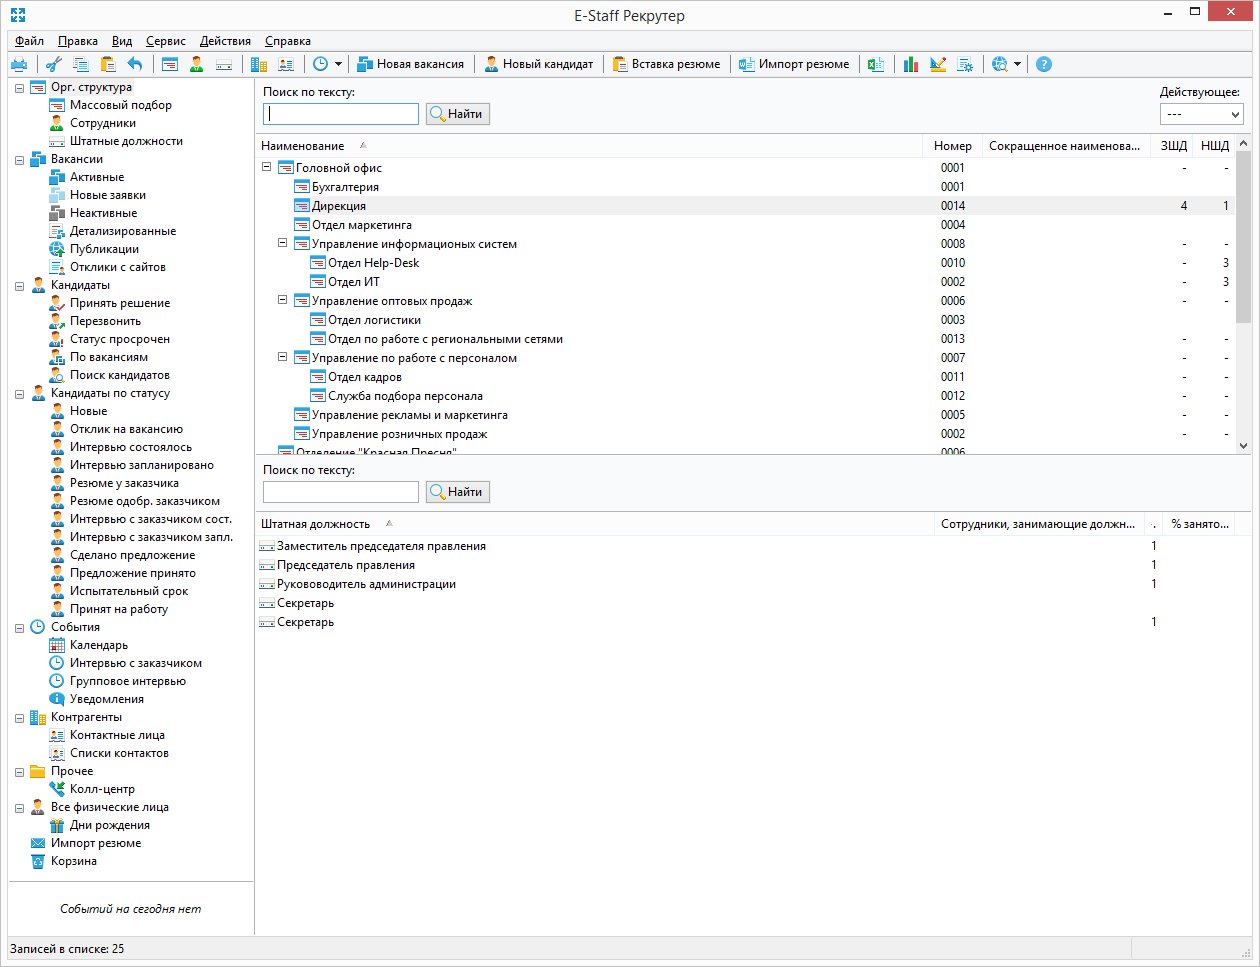
\includegraphics[scale=0.5]{e-staff-departments.png} 
	\caption{Управление подразделениями в системе E-Stuff}
	\label{fig:analysis:analogues:e-staff-departments}
\end{figure}

Также как и список подразделений, список сотрудников компании может автоматически синхронизироваться с системой
кадрового учета компании (1С, БОСС-Кадровик, SAP и др.) (рисунок~\ref{fig:analysis:analogues:e-staff-employees}).

\begin{figure}[!h]
	\centering
	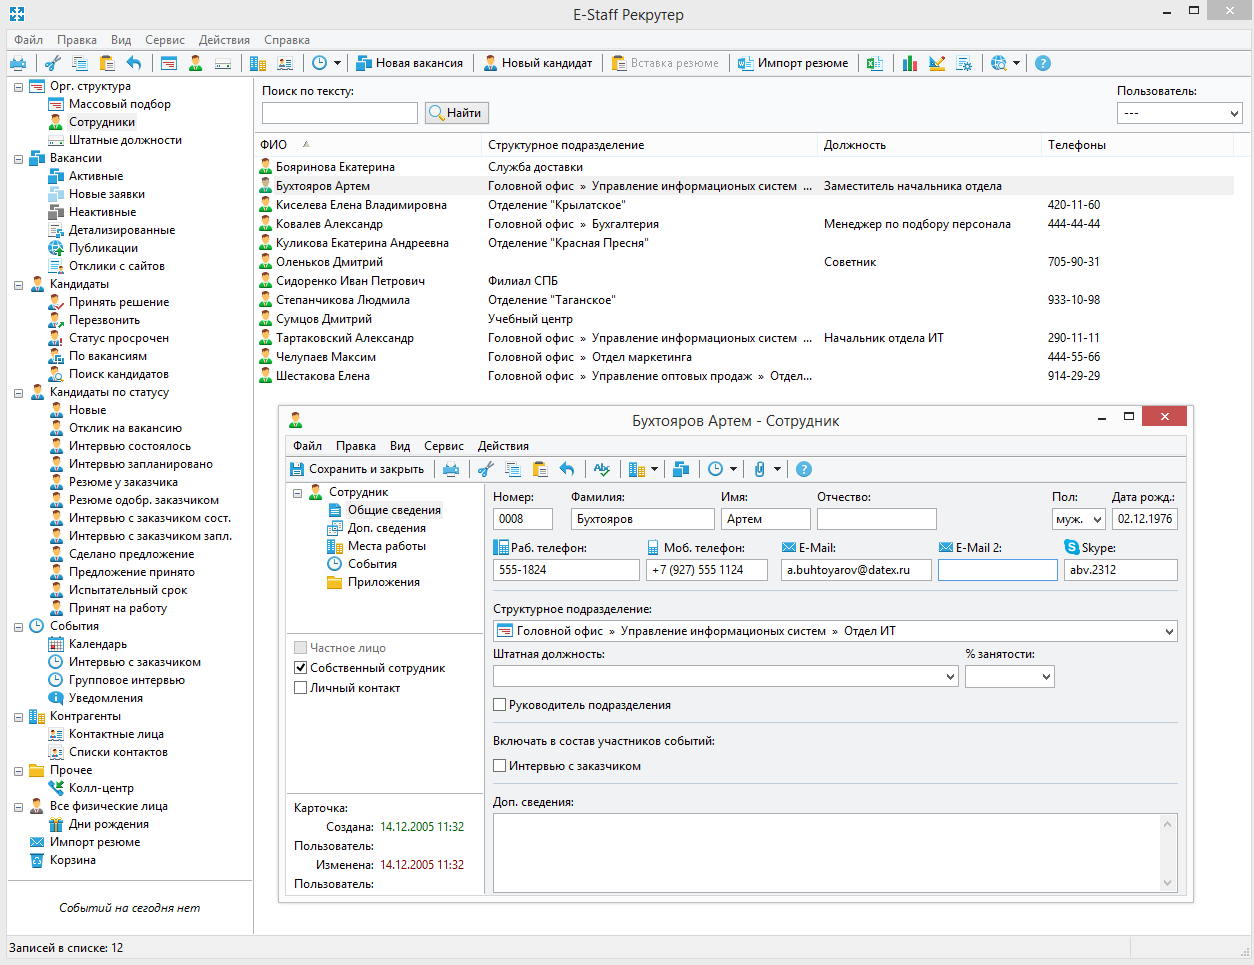
\includegraphics[scale=0.5]{e-staff-employees.png} 
	\caption{Управление сотрудниками в системе E-Stuff}
	\label{fig:analysis:analogues:e-staff-employees}
\end{figure}

Преимущества системы:
\begin{itemize}
	\item хранение данных о структуре и сотрудниках компании;
	\item работа с вакансиями компании;
	\item импорт данных из сторонних систем;
	\item поиск резюме в сети Интернет.
\end{itemize}

Недостатки системы:
\begin{itemize}
	\item ПО требует приобретения;
	\item устаревший интерфейс;
	\item отсутсвие кроссплатформенности.
\end{itemize}

1.2.1.2 1С:Зарплата и управление персоналом

1С:Зарплата и управление персоналом -- программа массового назначения, позволяющая в комплексе автоматизировать
задачи, связанные с расчетом заработной платы персонала и реализацией кадровой политики, с учетом требований
законодательства и реальной практики работы предприятий. Она может успешно применяться в службах управления персоналом
и бухгалтериях предприятий, а также в других подразделениях, заинтересованных в эффективной организации работы
сотрудников, для управления человеческими ресурсами коммерческих предприятий различного масштаба
(рисунок~\ref{fig:analysis:analogues:1c}).

В 1С:Зарплате и управлении персоналом поддерживаются все основные процессы управления персоналом, а также процессы
кадрового учета, расчета зарплаты, исчисления налогов, формирования отчетов и справок в государственные органы и
социальные фонды, планирования расходов на оплату труда. Учтены требования законодательства, реальная практика работы
предприятий и перспективные мировые тенденции развития подходов к управлению персоналом.

Кадровый учет обязателен для любой компании. С каждым годом он все более регламентируется законодательством, поэтому
возможность его автоматизации важна для многих компаний, особенно с большим штатом сотрудников
(рисунок~\ref{fig:analysis:analogues:1c_employees}).

\begin{figure}[!h]
	\centering
	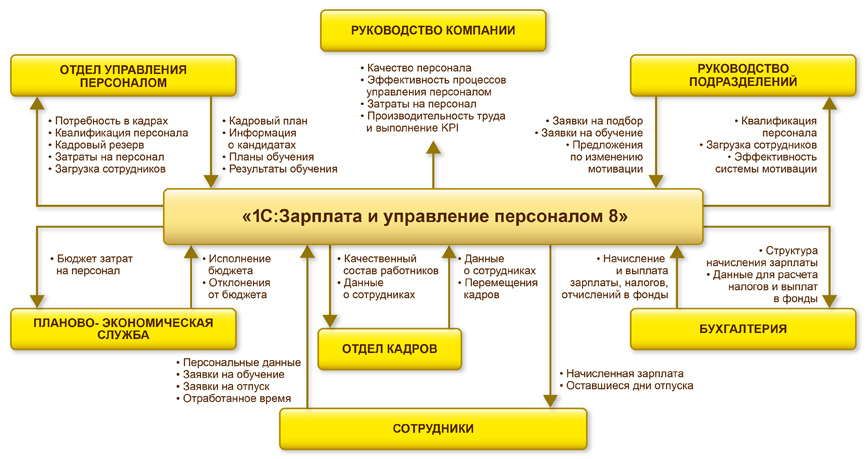
\includegraphics[scale=0.5]{1c.jpg} 
	\caption{Основные функции системы 1С:Зарплата и управление персоналом}
	\label{fig:analysis:analogues:1c}
\end{figure}

\begin{figure}[!h]
	\centering
	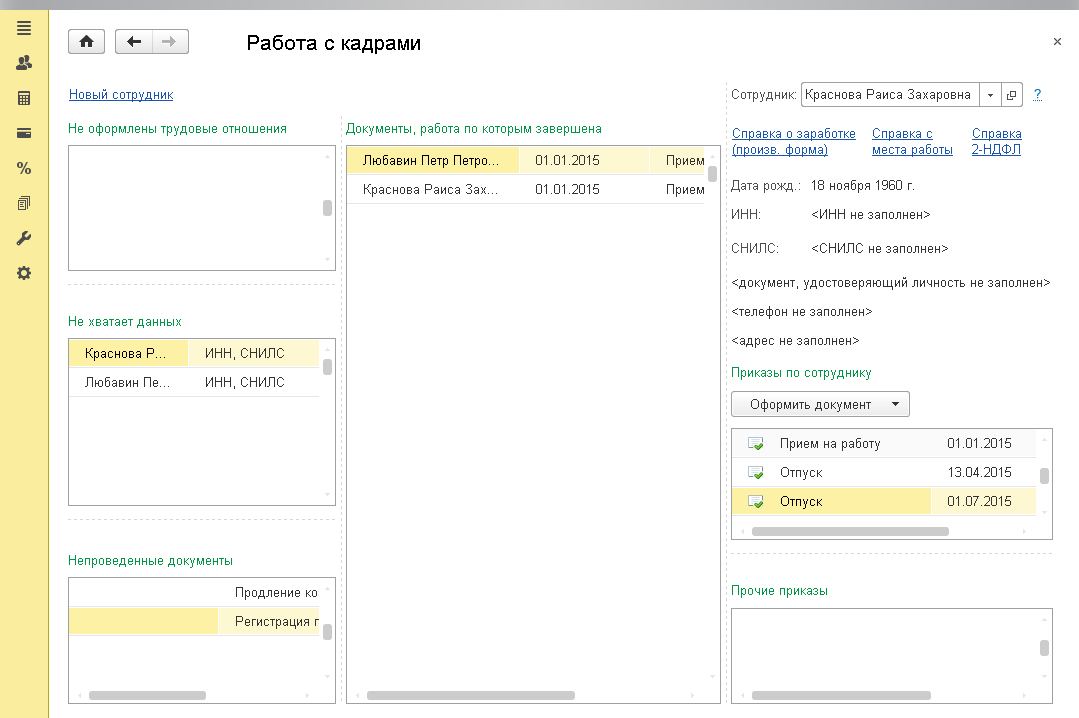
\includegraphics[scale=0.55]{1c_employees.png} 
	\caption{Кадровый учет в системе 1С:Зарплата и управление персоналом}
	\label{fig:analysis:analogues:1c_employees}
\end{figure}

«1С:Зарплата и управление персоналом 8» позволяет:
\begin{itemize}
	\item снизить временные затраты на выполнение кадровой работы;
	\item учитывать движение кадров;
	\item вести учет персональных данных работников;
	\item осуществлять воинский учет;
	\item вести учет рабочего времени;
	\item вести штатное расписание.
\end{itemize}

Преимущества системы:
\begin{itemize}
	\item возможность автоматизации расчета зарплаты;
	\item учет движения кадров;
	\item учет рабочего времени;
	\item возможность учета персональных данных работников.
\end{itemize}

Недостатки системы:
\begin{itemize}
	\item ПО требует приобретения;
	\item устаревший интерфейс;
	\item отсутсвие кроссплатформенности;
	\item сложность использования;
	\item необходимость предварительного обучения персонала.
\end{itemize}
\pagebreak

\subsubsection{} Генерация резюме
\label{sec:analysis:analogues:generation}

В настоящее время практика направления кандидатом, ведущим поиск работы, своего резюме работодателю или компании по
подбору персонала в ответ на его объявление о вакансии находит все большее распространение не только среди
многонациональных, но и беларуских компаний. Представление резюме потенциальному работодателю или агентству по подбору
персонала становится одним из основных методов трудоустройства для квалифицированных кандидатов.

Резюме -- это документ, в котором в краткой, но емкой форме изложены основные сведения о профессиональных умениях и
навыках, трудовой биографии и личных данных кандидата. Оно позволяет работодателю заочно, с минимальными затратами
времени ознакомиться в первом приближении с деловыми и личностными качествами кандидатов, произвести первичный отбор
наиболее достойных и дать первую оценку их соответствия имеющейся вакансии.

Практика показывает, что в большинстве случаев специалист по подбору персонала или менеджер по работе с персоналом при
принятии решения о том, пригласить кандидата на интервью или нет, основывается на содержании и форме резюме \cite{cv}.

Принято считать, что профессионально составленное резюме обычно содержит следующие разделы:
\begin{itemize}
	\item общие данные о кандидате — возраст, адрес проживания, контактная информация;
	\item образование — как основное, так и дополнительное;
	\item профессиональные умения и навыки;
	\item трудовая биография в обратном хронологическом порядке (последнее место работы — сначала);
	\item личные данные о кандидате, его увлечения;
	\item пожелания кандидата относительно будущей должности, уровня компенсации, возможного района или региона работы.
\end{itemize}

Cуществует несколько сервисов, автоматизирующих процесс генерации резюме. В процессе проектирования
системы были изучены следующие существующие аналоги:
\begin{itemize}
	\item cистема генерации резюме CVMaker;
	\item cистема визулизации резюме Vizualize.
\end{itemize}

1.2.2.1 Cистема генерации резюме CVMaker

Cистема позволяет пользователям автоматически генерировать резюме(рисунок~\ref{fig:analysis:analogues:cvmaker}).
CVMaker дает на выбор 6 бесплатных шаблонов для резюме, выполненных в строгом классическом стиле. Однако система никак
не связана с компанией и не позволяет управлять уже созданными резюме.

Преимущества:
\begin{itemize}
	\item бесплатность;
	\item возможность выбора шаблона;
	\item Возможность выбора формата загрузки.
\end{itemize}

Недостатки:
\begin{itemize}
	\item отсутствие связи с компанией;
	\item невозможность проверки заполненного резюме сотрудником компании встроенными средствами;
	\item невозможность корректировки уже сгенерированного резюме.
\end{itemize}

\begin{figure}[!t]
	\centering
	
\includegraphics[scale=0.7]{cvmaker.png} 
	\caption{Пример готового резюме в системе СVMaker}
	\label{fig:analysis:analogues:cvmaker}
\end{figure}

1.2.2.2 Cистема визулизации резюме Vizualize

Скучные списки о прошлых местах работы, заслугах и навыках можно превратить в интересную инфографику на
Vizualize(рисунок~\ref{fig:analysis:analogues:visualize}). Чтобы создать ее, нужен профиль в LinkedIn. Информацию можно
импортировать также из Twitter, Facebook и Foursquare.

\begin{figure}[!t]
	\centering
	
\includegraphics[scale=0.5]{visualize.png} 
	\caption{Стартовая страница Visualize}
	\label{fig:analysis:analogues:visualize}
\end{figure}

Преимущества:
\begin{itemize}
	\item бесплатность;
	\item визуализация резюме;
	\item возможность импорта данных из социальных сетей.
\end{itemize}

Недостатки:
\begin{itemize}
	\item отсутствие связи с компанией;
	\item невозможность проверки заполненного резюме сотрудником компании встроенными средствами;
	\item невозможность вывода резюме на бумажный носитель.
\end{itemize}


\subsection{Требования к проектируемому программному средству}
\label{sec:analysis:specification}

По результатам изучения предметной области, анализа литературных источников и обзора существующих систем-аналогов
сформулируем требования к проектируемому программному средству.
\pagebreak

\subsubsection{} Назначение проекта
\label{sec:analysis:specification:purpose}

Назначением проекта является разработка программного средства, обеспечивающего отслеживание
активных вакансии в компании, текущую занятость сотрудников на проектах, их способности, а также автоматическая генерация
на основе полученных данных резюме сотрудника для дальнейшего использования в отделе маркетинга и продаж.

\subsubsection{} Основные функции
\label{sec:analysis:specification:functions}

Программное средство должно поддерживать следующие основные фун\-к\-ции:

\begin{itemize}
	\item регистрация и аутентификация;
	\item возможность приглашения пользователей;
	\item поддержка системы ролей;
	\item управление проектами организации;
	\item управление отделами организации;
	\item управление должностями;
	\item управление профилями пользователей;
	\item управление вопросами для генерации резюме;
	\item генерация резюме;
	\item возможность проверки резюме другими сотрудниками организации;
	\item уведомление сотрудников о необходимости проверки резюме.
\end{itemize}

\subsubsection{} Требования к входным данным
\label{sec:analysis:specification:inputs}

Входные данные для программного средства должны быть представлены в виде вводимого пользователем с помощью клавиатуры
текста и выбора доступных опций пользовательского интерфейса.

Должны быть реализованы проверки вводимых данных на корректность с отображением информации об ошибках в случае их
некорректности.

\subsubsection{} Требования к выходным данным
\label{sec:analysis:specification:outputs}

Выходные данные программного средства должны быть представлены посредством отображения информации с помощью различных
элементов пользовательского интерфейса.

\subsubsection{} Требования к временным характеристикам
\label{sec:analysis:specification:timing}

Производительность программно-аппаратного комплекса должна обеспечивать следующие временные характеристики: время
реакции не запрос пользователя не должно превышать 2 секунд при минимальной скорости соединения 10 МБит/с. Допускается
невыполнение данного требования в случае, когда невозможность обеспечить заявленную производительность обусловлена
объективными внешними причинами.

\subsubsection{} Требования к надежности
\label{sec:analysis:specification:reliability}

Надежное функционирование программы должно быть обеспечено выполнением следующих организационно-технических мероприятий:

\begin{itemize}
	\item организация бесперебойного питания;
	\item выполнение рекомендаций Министерства труда и социальной защиты РБ, изложенных в Постановлении от 23 марта 2011 г. «Об утверждении Норм времени на работы по обслуживанию персональных электронно-вы\-числи\-тельных машин, организационной техники и офисного оборудования»;
	\item выполнение требований ГОСТ 31078-2002 <<Защита информации. Испытания программных средств на наличие компьютерных вирусов>>;
	\item необходимым уровнем квалификации пользователей.
\end{itemize}


Время восстановления после отказа, вызванного сбоем электропитания технических средств (иными внешними факторами),
нефатальным сбоем операционной системы, не должно превышать времени, необходимого на перезагрузку операционной системы
и запуск программы, при условии соблюдения условий эксплуатации технических и программных средств. Время восстановления
после отказа, вызванного неисправностью технических средств, фатальным сбоем операционной системы, не должно
превышать времени, требуемого на устранение неисправностей технических средств и переустановки программных средств.

Отказы программы возможны вследствие некорректных действий пользователя при взаимодействии с операционной системой.
Во избежание возникновения отказов программы по указанной выше причине следует обеспечить работу конечного
пользователя без предоставления ему административных привилегий.

\subsubsection{} Требования к аппаратному обеспечению серверной части
\label{sec:analysis:specification:server_requirments}

ЭВМ, на которой должна функционировать серверная часть программного средства, должна обладать следующими
минимальными характеристиками:

\begin{itemize}
	\item процессор Intel Core i5 с тактовой частотой 2 ГГц;
	\item жесткий диск объемом 100 Гб;
	\item оперативная память 4 Гб;
	\item сетевая карта Ethernet 100 МБит/с.
\end{itemize}

Также для функционирования серверной части требуется установленный Ruby on Rails сервер, который работает на
операционной системе Linux.

\subsubsection{} Требования к аппаратному обеспечению клиентской части
\label{sec:analysis:specification:client_requirments}

Клиентская часть программного средства должна функционировать на ЭВМ со следующими минимальными характеристиками:

\begin{itemize}
	\item процессор Intel Сeleron с тактовой частотой 2 ГГц и более;
	\item оперативная память 4 Гб и более;
	\item возножность выхода в сеть Интернет.
\end{itemize}

Для корректной работы программного средства необходим один из следующих браузеров с соответствующей минимальной версией:

\begin{itemize}
	\item Google Chrome 70;
	\item Opera 58;
	\item Mozilla Firefox 66;
	\item Apple Safari 12.0;
	\item Microsoft Edge 44.
\end{itemize}

\subsubsection{} Выбор технологий программирования
\label{sec:analysis:specification:language}

Язык программирования, на котором будет реализована система, заслуживает большого внимания, так как вы будете
погружены в него с начала конструирования программы до самого конца. Исследования показали, что выбор языка
программирования несколькими способами влияет на производительность труда программистов и качество создаваемого ими
кода. Если язык хорошо знаком программистам, они работают более производительно. Данные, полученные при помощи модели
оценки Cocomo II, показывают, что программисты, использующие язык, с которым они работали три года или более, примерно
на 30\% более продуктивны, чем программисты, обладающие аналогичным опытом, но для которых язык является
новым~\cite{software_cost_estimation}. В более раннем исследовании, проведенном в IBM, было обнаружено, что
программисты, обладающие богатым опытом использования языка программирования, были более чем втрое
производительнее программистов, имеющих минимальный опыт~\cite{method_of_programming_measurement_and_estimation}.

JavaScript ("JS" для краткости) — это полноценный динамический язык программирования, который применяется к HTML
документу, и может обеспечить динамическую интерактивность на веб-сайтах.

JavaScript сам по себе довольно компактный, но очень гибкий. Разработчиками написано большое количество инструментов
поверх основного языка JavaScript, которые разблокируют огромное количество дополнительных функций с очень
небольшим усилием. К ним относятся:

\begin{itemize}
	\item программные интерфейсы приложения (API), встроенные в браузеры, обеспечивающие различные функциональные
	возможности, такие как динамическое создание HTML и установку CSS стилей, захват и манипуляция видеопотоком, работа с
	веб-камерой пользователя или генерация 3D графики;
	\item сторонние API позволяют разработчикам внедрять функциональ\-ность в свои сайты от других разработчиков,
	таких как Twitter или Facebook;
	\item также есть возможность применить к HTML сторонние фреймворки и библиотеки, что позволит ускорить создание
	сайтов и приложений~\cite{javascript_basics}.
\end{itemize}

Выбранный язык программирования является средством для программирования клиентской части приложения.
Поскольку для приложения в любом случае понадобится база данных, то есть два варианта:

\begin{itemize}
	\item осуществлять запросы к БД напрямую с клиентского приложения;
	\item реализовать серверную прослойку между клиентской частью и базой данных.
\end{itemize}

Первый подход крайне небезопасен: очень опасно предоставлять открытый доступ к БД. В это же время, второй способ,
помимо ее сокрытия, предоставляет возможность проверки подлинности и предоставления прав пользователям.
В связи с этим появляется проблема выбора технологий для серверной части. Основным влияющим фактором является
имеющийся опыт команды разработки, в связи с чем была выбрана технология Ruby on Rails и язык программирования Ruby.

Язык программирования Ruby, является кроссплатформенным языком программирования. Ruby -- это тщательно сбалансированный
язык. Его создатель Юкихиро Мацумото, объединил части его любимых языков (Perl, \linebreak Smalltalk, Eiffel, Ada и Lisp) чтобы
сформировать новый язык, в котором парадигма функционального программирования сбалансирована принципами
императивного программирования. 

В Ruby всё -- объект. Для каждой частицы информации или кода могут быть определены собственные свойства и действия.
В объектно-ориентирован\-ном программировании свойства называются переменными объекта, а действия – методами.
Чистейший объектно-ориентированный подход Ruby может быть продемонстрирован парой строк кода, в которых производится
действие над числом.

Во многих языках числа и другие примитивные типы данных не являются объектами. Ruby под влиянием языка Smalltalk
позволяет задать методы и переменные объекта всем типам данных. Это упрощает использование Ruby, так как правила
применимые к объектам -- применимы ко всему Ruby~\cite{ruby}.

Ruby on Rails - фреймворк для веб-разработки, написанный на языке программирования Ruby. Он разработан, чтобы сделать
программирование веб-приложений проще, так как использует ряд допущений о том, что нужно каждому разработчику для
создания нового проекта. Он позволяет писать меньше кода в процессе программирования, в сравнении с другими языками и
фреймворками. Ruby on Rails реализует архитектурный шаблон Model-View-Controller, представленный на
рисунке~\ref{fig:analysis:specification:language:mvc} для веб-приложений, а также
обеспечивает их интеграцию с веб-сервером и сервером баз данных.

\begin{figure}[!h]
	\centering
	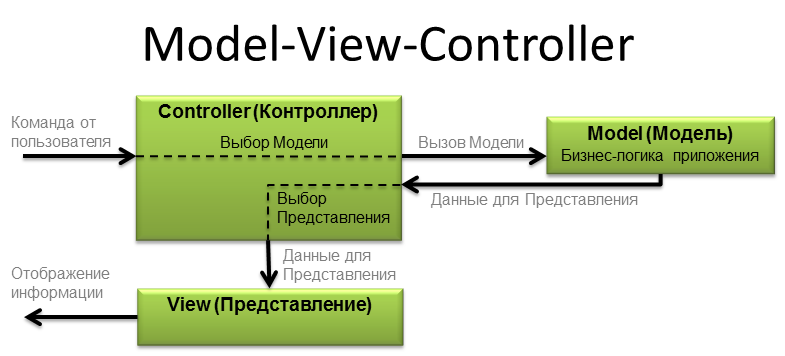
\includegraphics[scale=0.6]{mvc.png} 
	\caption{архитектурный шаблон Model-View-Controller}
	\label{fig:analysis:specification:language:mvc}
\end{figure}

Философия Rails включает два важных принципа:

\begin{itemize}
	\item Don't Repeat Yourself: DRY -- это принцип разработки ПО, который гласит, что "Каждый кусочек информации должен
	иметь единственное, неизбыточное, авторитетное представление в системе." Не пишите одну и ту же информацию снова и
	снова, код будет легче поддерживать, и он будет более расширяемым и менее ошибочным;
	\item Convention Over Configuration: у Rails есть мнения о наилучших способах делать множество вещей в веб-приложении,
	и по умолчанию выставлены эти соглашения, вместо того, чтобы заставлять вас по мелочам править многочисленные
	конфигурационные файлы~\cite{rails}.
\end{itemize}

По результатам обзора возможных платформ, представленных в пункте 1.1.2, было принято решение выбрать основной для
разработки платформу веб-приложений.

В качестве СУБД было принято решение использовать PostgreSQL - свободно распространяемую объектно-реляционную систему
управления базами данных, которая является наиболее развитой из открытых СУБД в мире и являющаяся реальной
альтернативой коммерческим базам данных.

Надежность PostgreSQL является проверенным и доказанным фактом и обеспечивается следующими возможностями:

\begin{itemize}
	\item полное соответствие принципам ACID -- атомарность, непротиворечивость, изолированность, сохранность данных.
	Атомарность -- транзакция рассматривается как единая логическая единица, все ее изменения или сохраняются целиком,
	или полностью откатываются. Непротиворечивость -- транзакция переводит базу данных из одного непротиворечивого
	состояния (на момент старта транзакции) в другое непротиворечивое состояние (на момент завершения транзакции).
	Непротиворечивым считается состояние базы, когда выполняются все ограничения физической и логической целостности
	базы данных, при этом допускается нарушение ограничений целостности в течение транзакции, но на момент завершения все
	ограничения целостности, как физические, так и логические, должны быть соблюдены. Изолированность -- изменения данных
	при конкурентных транзакциях изолированы друг от друга на основе системы версионности.
	Сохранность данных -- PostgreSQL заботится о том, что результаты успешных транзакций гарантировано сохраняются на
	жесткий диск вне зависимости от сбоев аппаратуры;
	\item многоверсионность используется для поддержания согласованности данных в конкурентных условиях, в то время как в
	традиционных базах данных используются блокировки. многоверсионность означает, что каждая транзакция видит копию
	данных (версию базы данных) на время начала транзакции, несмотря на то, что состояние базы могло уже измениться;
	\item репликация также повышает надежность PostgreSQL;
	\item открытость кодов PostgreSQL означает их абсолютную доступность для любого, а либеральная BSD лицензия не
	накладывает никаких ограничений на использование кода.
\end{itemize}

Производительность PostgreSQL основывается на использовании индексов, интеллектуальном планировщике запросов,
тонкой системы блокировок, системе управления буферами памяти и кэширования, превосходной масштабируемости при
конкурентной работе~\cite{postgres}.

Сформулированные требования позволят осуществить успешное проектирование и разработку программного средства.

